\section{Part B: Text classification of Wikipage entries}
\label{part2}
The details of the dataset are given as follows:
\begin{quote}
The dataset used in this project contains the first paragraphs collected from Wikipage entries and the corresponding labels about their category. You will implement CNN and RNN layers at the word and character levels for the classification of texts in the paragraphs. The output layer of the networks is a softmax layer. The training and test datasets will be read from 'train\_medium.csv and 'test\_medium.csv' files. The training dataset contains 5600 entries and test dataset contains 700 entries. The label of an entry is one of the 15 categories such as people, company, schools, etc. The input data is in text, which should be converted to character/word IDs to feed to the networks by using 'tf.contrib.learn.preprocessing'. Restrict the maximum length of the characters/word inputs to 100. Use the Adam optimizer for training with a batch size = 128 and learning rate = 0.01. Assume there are 256 different characters.
\end{quote}

The character and word CNN is defined as in Listing \ref{ls:2_cnn}, while the char and word RNN is defined as in Listing \ref{ls:2_rnn}, with the loss and accuracy functions defined in Listing \ref{ls:2_cost}.

\begin{lstlisting}[language=Python, caption= Character and word convolutional neural network (layers controlled by layers parameter), label=ls:2_cnn]
def cnn_model(x, model_type, dropout=False):
    if model_type == 'char':
        input_layer = tf.reshape(
            tf.one_hot(x, 256), [-1, MAX_DOCUMENT_LENGTH, 256, 1])

        # if dropout:
        #     input_layer = tf.layers.dropout(input_layer, 0.1)

        with tf.variable_scope('Char_CNN_Layer1'):
            conv1 = tf.layers.conv2d(
                input_layer,
                filters=N_FILTERS,
                kernel_size=FILTER_SHAPE1,
                padding='VALID',
                activation=tf.nn.relu)
            pool1 = tf.layers.max_pooling2d(
                conv1,
                pool_size=POOLING_WINDOW,
                strides=POOLING_STRIDE,
                padding='SAME')
            if dropout:
                pool1 = tf.layers.dropout(pool1, 0.25)
        with tf.variable_scope('Char_CNN_Layer2'):
            conv2 = tf.layers.conv2d(
                pool1,
                filters=N_FILTERS,
                kernel_size=FILTER_SHAPE2,
                padding='VALID',
                activation=tf.nn.relu)
            pool2 = tf.layers.max_pooling2d(
                conv2,
                pool_size=POOLING_WINDOW,
                strides=POOLING_STRIDE,
                padding='SAME')
            if dropout:
                pool2 = tf.layers.dropout(pool2, 0.25)

        pool2 = tf.squeeze(tf.reduce_max(pool2, 1), squeeze_dims=[1])

        logits = tf.layers.dense(pool2, MAX_LABEL, activation=None)

        # if dropout:
        #     logits = tf.layers.dropout(logits, 0.5)

        return input_layer, logits
    
    elif model_type == 'word':
        word_vectors = tf.contrib.layers.embed_sequence(
        x, vocab_size=n_words, embed_dim=EMBEDDING_SIZE)
        
        word_list = tf.unstack(word_vectors, axis=1)

        input_layer = tf.reshape(
            word_vectors, [-1, MAX_DOCUMENT_LENGTH, HIDDEN_SIZE, 1])
        # if dropout:
        #     input_layer = tf.layers.dropout(input_layer, 0.1)

        with tf.variable_scope('Word_CNN_Layer1'):
            conv1 = tf.layers.conv2d(
                input_layer,
                filters=N_FILTERS,
                kernel_size=[20, 20],
                padding='VALID',
                activation=tf.nn.relu)
            pool1 = tf.layers.max_pooling2d(
                conv1,
                pool_size=POOLING_WINDOW,
                strides=POOLING_STRIDE,
                padding='SAME')
            if dropout:
                pool1 = tf.layers.dropout(pool1, 0.25)
        with tf.variable_scope('Word_CNN_Layer2'):
            conv2 = tf.layers.conv2d(
                pool1,
                filters=N_FILTERS,
                kernel_size=FILTER_SHAPE2,
                padding='VALID',
                activation=tf.nn.relu)
            pool2 = tf.layers.max_pooling2d(
                conv2,
                pool_size=POOLING_WINDOW,
                strides=POOLING_STRIDE,
                padding='SAME')
            if dropout:
                pool2 = tf.layers.dropout(pool2, 0.25)

        pool2 = tf.squeeze(tf.reduce_max(pool2, 1), squeeze_dims=[1])

        logits = tf.layers.dense(pool2, MAX_LABEL, activation=None)

        # if dropout:
        #     logits = tf.layers.dropout(logits, 0.5)

        return input_layer, logits
    else:
        raise Exception(f'No model type named {model_type}')
\end{lstlisting}

\begin{lstlisting}[language=Python, caption= Character and word recurrent neural network neural network (layers controlled by layers parameter), label=ls:2_rnn]
def rnn_model(x, model_type, cell_type='GRU', num_layers=1, dropout=False):
    if model_type == 'char':
        input_layer = tf.one_hot(x, 256)
        input_layer = tf.unstack(input_layer, axis=1)

        cells_ = []
        for i in range(num_layers):
            # Define cell type
            if cell_type == 'GRU':
                cell = tf.nn.rnn_cell.GRUCell(HIDDEN_SIZE, reuse=tf.get_variable_scope().reuse)
            elif cell_type == 'VANILLA':
                cell = tf.nn.rnn_cell.BasicRNNCell(HIDDEN_SIZE, reuse=tf.get_variable_scope().reuse)
            elif cell_type == 'LSTM':
                cell = tf.nn.rnn_cell.LSTMCell(HIDDEN_SIZE, reuse=tf.get_variable_scope().reuse)
            else:
                raise Exception(f'No cell type matches {cell_type}')

            # Define dropout
            if dropout:
                cell = tf.nn.rnn_cell.DropoutWrapper(cell, output_keep_prob=0.5)

            cells_.append(cell)

        # Multi-layer rnn cells
        cells = tf.nn.rnn_cell.MultiRNNCell(cells_)
        _, encoding = tf.nn.static_rnn(cells, input_layer, dtype=tf.float32)

        encoding = np.array(encoding).flatten()

        # Dense layer
        logits = tf.layers.dense(encoding[-1], MAX_LABEL, activation=None)
        # if dropout:
        #     logits = tf.layers.dropout(logits, 0.5)

        return input_layer, logits

    elif model_type == 'word':
        word_vectors = tf.contrib.layers.embed_sequence(
            x, vocab_size=n_words, embed_dim=EMBEDDING_SIZE)

        word_list = tf.unstack(word_vectors, axis=1)

        cells_ = []
        for i in range(num_layers):
            # Define cell type
            if cell_type == 'GRU':
                cell = tf.nn.rnn_cell.GRUCell(HIDDEN_SIZE, reuse=tf.get_variable_scope().reuse)
            elif cell_type == 'VANILLA':
                cell = tf.nn.rnn_cell.BasicRNNCell(HIDDEN_SIZE, reuse=tf.get_variable_scope().reuse)
            elif cell_type == 'LSTM':
                cell = tf.nn.rnn_cell.LSTMCell(HIDDEN_SIZE, reuse=tf.get_variable_scope().reuse)
            else:
                raise Exception(f'No cell type matches {cell_type}')

            # Define dropout
            if dropout:
                cell = tf.nn.rnn_cell.DropoutWrapper(cell, output_keep_prob=0.5)

            cells_.append(cell)

        # Multi-layer rnn cells
        cells = tf.nn.rnn_cell.MultiRNNCell(cells_)
        _, encoding = tf.nn.static_rnn(cells, word_list, dtype=tf.float32)

        encoding = np.array(encoding).flatten()

        # Dense layer
        logits = tf.layers.dense(encoding[-1], MAX_LABEL, activation=None)

        # if dropout:
        #     logits = tf.layers.dropout(logits, 0.5)

        return word_list, logits
    else:
        raise Exception(f'No model type named {model_type}')
\end{lstlisting}

\begin{lstlisting}[language=Python, caption= loss and accuracy functions, label=ls:2_cost]
def create_model(feature_size, neuron_size, weight_decay_beta, learning_rate, layers=3, dropout=False):
# Create the model
x = tf.placeholder(tf.int64, [None, MAX_DOCUMENT_LENGTH])
y_ = tf.placeholder(tf.int64)

inputs, logits = rnn_model(x, model_type='char', cell_type=item['cell_type'], num_layers=item['num_layers'])

# Optimizer
entropy = tf.reduce_mean(tf.nn.softmax_cross_entropy_with_logits_v2(labels=tf.one_hot(y_, MAX_LABEL), logits=logits))

# Gradient clipping
if item['grad_clip']:
    minimizer = tf.train.AdamOptimizer()
    grads_and_vars = minimizer.compute_gradients(entropy)
    grad_clipping = tf.constant(2.0, name="grad_clipping")
    clipped_grads_and_vars = []
    for grad, var in grads_and_vars:
        clipped_grad = tf.clip_by_value(grad, -grad_clipping, grad_clipping)
        clipped_grads_and_vars.append((clipped_grad, var))
    train_op = minimizer.apply_gradients(clipped_grads_and_vars)
else:
    train_op = tf.train.AdamOptimizer(lr).minimize(entropy)

correct_prediction = tf.equal(tf.argmax(logits, 1), y_)
correct_prediction = tf.cast(correct_prediction, tf.float32)
accuracy = tf.reduce_mean(correct_prediction)
\end{lstlisting}

Mini-batch gradient descend is done through Listing \ref{ls:mini_batch}.

\begin{lstlisting}[language=Python, caption= Mini-batch setup, label=ls:mini_batch]
for start, end in zip(range(0, len(train_X), batch_size), range(batch_size, len(train_X), batch_size)):
    _, batch_cost = sess.run([train_step, loss], {x: train_X[start:end], y_: train_Y[start:end]})
    train_cost_.append(batch_cost)
\end{lstlisting}

\subsection{Question 1}
\label{2q1}
\begin{quote}
Design a Character CNN Classifier that receives character ids and classifies the input. The CNN has two convolution and pooling layers:
\begin{itemize}
    \item A convolution layer $C_1$ of 10 filters of window size 20x256, VALID padding, and ReLU neurons. A max pooling layer $S_1$ with a pooling window of size 4x4, with stride = 2, and padding = 'SAME'.
    \item A convolution layer $C_2$ of 10 filters of window size 20x1, VALID padding, and ReLU neurons. A max pooling layer $S_2$ with a pooling window of size 4x4, with stride = 2 and padding = 'SAME'.
\end{itemize}
Plot the entropy cost on the training data and the accuracy on the testing data against training
epochs
\end{quote}

\begin{figure}[H]
    \begin{subfigure}{0.5\textwidth}
        \centering
        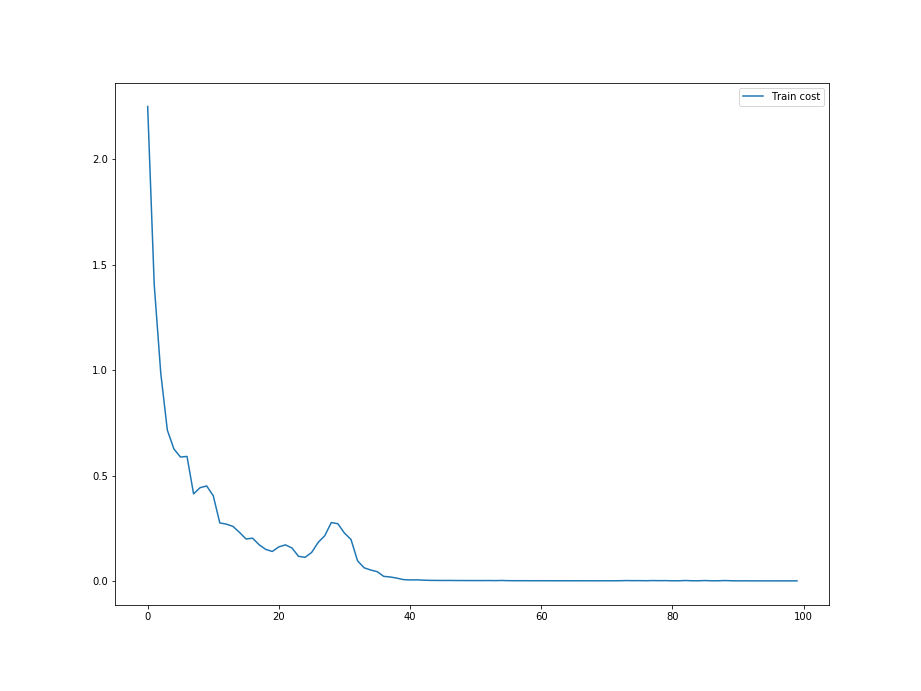
\includegraphics[width=1\linewidth]{assets/plots2/q1_1.png}
        \caption{Training cost against epochs for CNN}
    \end{subfigure}
    \begin{subfigure}{0.5\textwidth}
        \centering
        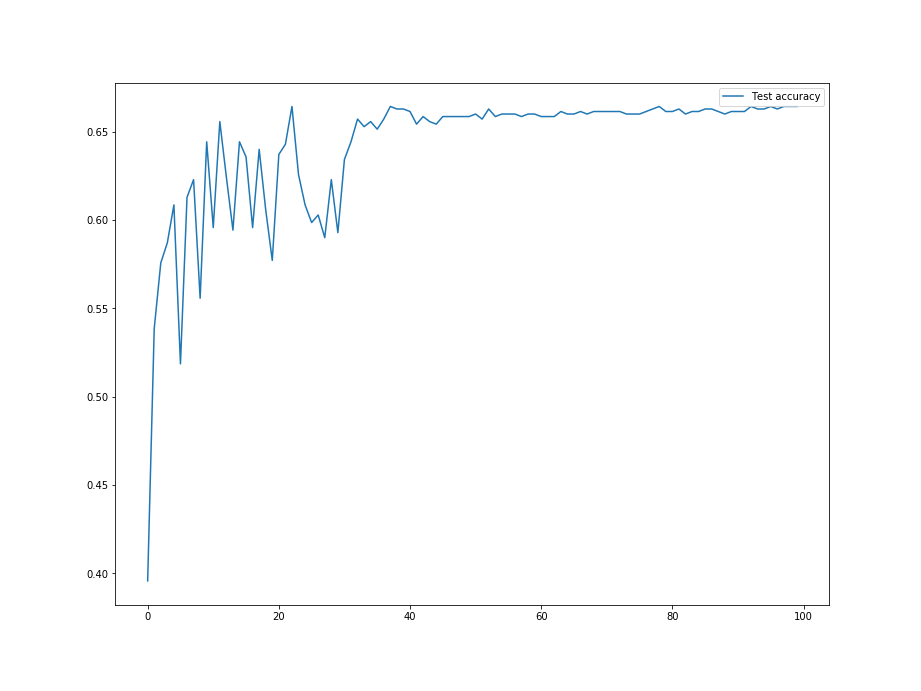
\includegraphics[width=1\linewidth]{assets/plots2/q1_2.png}
        \caption{Test accuracy against epochs for CNN}
    \end{subfigure}
    \caption{Plot of training cost and testing accuracy against epochs for character CNN}
    \label{fig:2_1}
\end{figure}

\subsection{Question 2}
\label{2q2}
\begin{quote}
Design a Word CNN Classifier that receives word ids and classifies the input. Pass the inputs
through an embedding layer of size 20 before feeding to the CNN. The CNN has two
convolution and pooling layers with the following characteristics:
\begin{itemize}
    \item A convolution layer $C_1$  of 10 filters of window size 20x20, VALID padding, and ReLU neurons. A max pooling layer $S_1$ with a pooling window of size 4x4, with stride = 2 and padding = 'SAME'.
    \item A convolution layer $C_2$ of 10 filters of window size 20x1, , VALID padding, and ReLU neurons. A max pooling layer $S_2$ with a pooling window of size 4x4, with stride = 2 and padding = 'SAME'.
\end{itemize}
Plot the entropy cost on the training data and the accuracy on the testing data against training epochs
\end{quote}
\begin{figure}[H]
    \begin{subfigure}{0.5\textwidth}
        \centering
        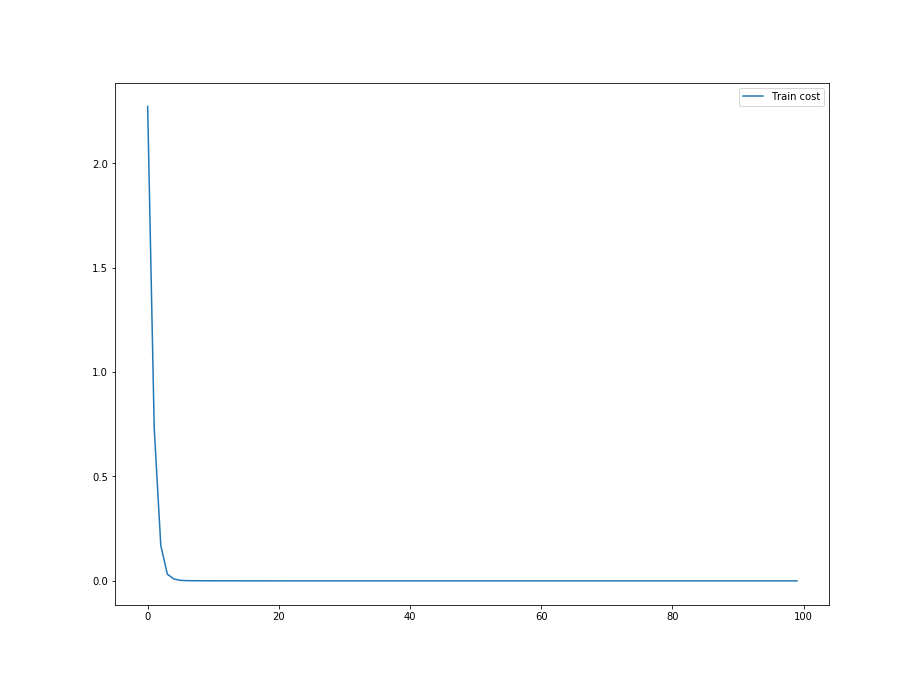
\includegraphics[width=1\linewidth]{assets/plots2/q2_1.png}
        \caption{Training cost against epochs for CNN}
        \label{fig:1a_cost}
    \end{subfigure}
    \begin{subfigure}{0.5\textwidth}
        \centering
        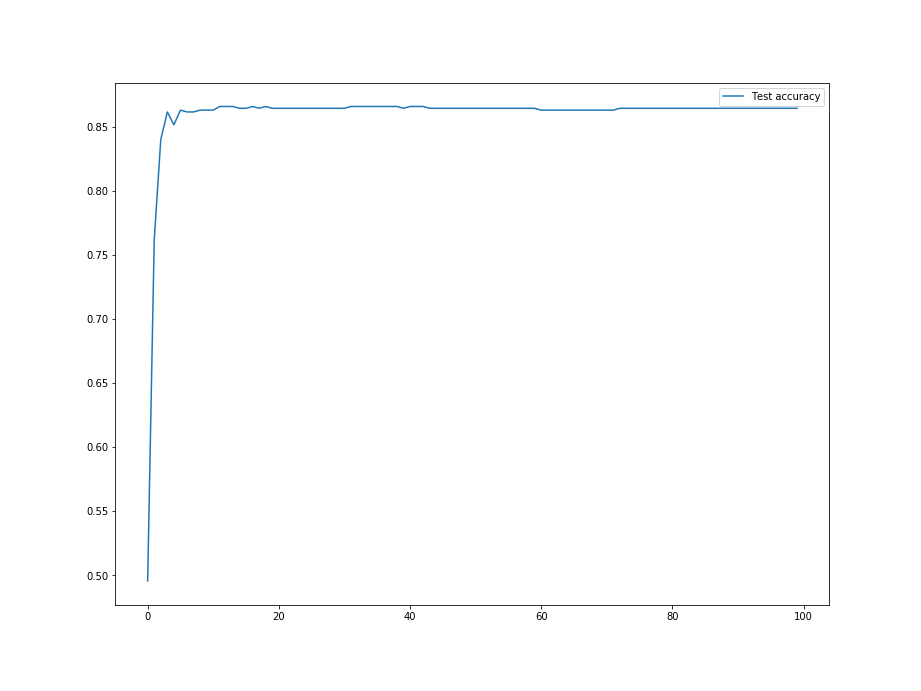
\includegraphics[width=1\linewidth]{assets/plots2/q2_2.png}
        \caption{Test accuracy against epochs for CNN}
        \label{fig:1a_cost}
    \end{subfigure}
    \caption{Plot of training cost and testing accuracy against epochs for word CNN}
    \label{fig:1a}
\end{figure}

\subsection{Question 3}
\label{2q3}
\begin{quote}
Design a Character RNN Classifier that receives character ids and classify the input. The RNN is GRU layer and has a hidden-layer size of 20. Plot the entropy cost on training data and the accuracy on testing data against training epochs.
\end{quote}

\begin{figure}[H]
    \begin{subfigure}{0.5\textwidth}
        \centering
        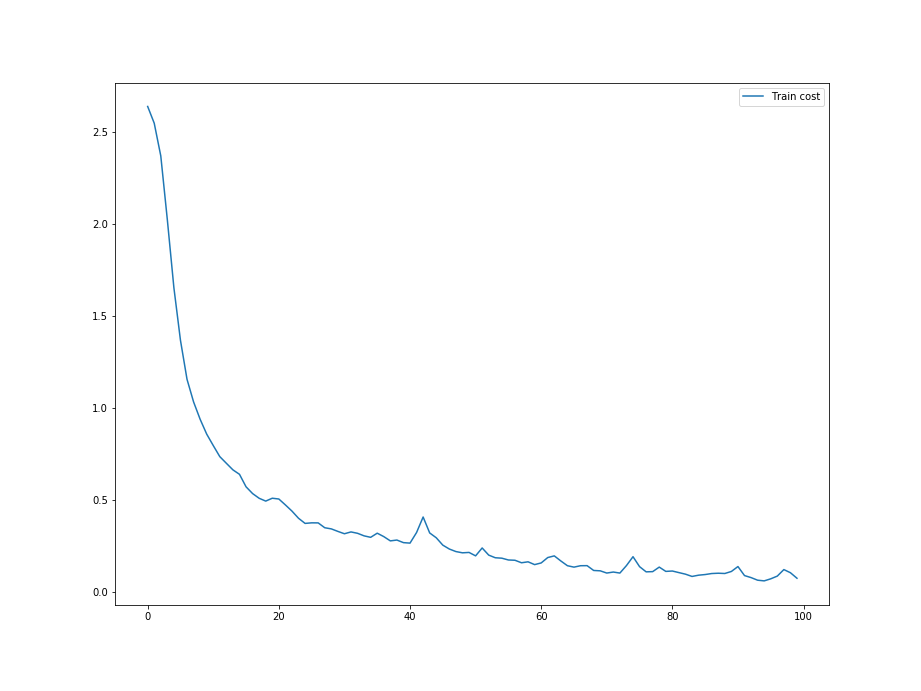
\includegraphics[width=1\linewidth]{assets/plots2/q3_1.png}
        \caption{Training cost against epochs for RNN}
        \label{fig:1a_cost}
    \end{subfigure}
    \begin{subfigure}{0.5\textwidth}
        \centering
        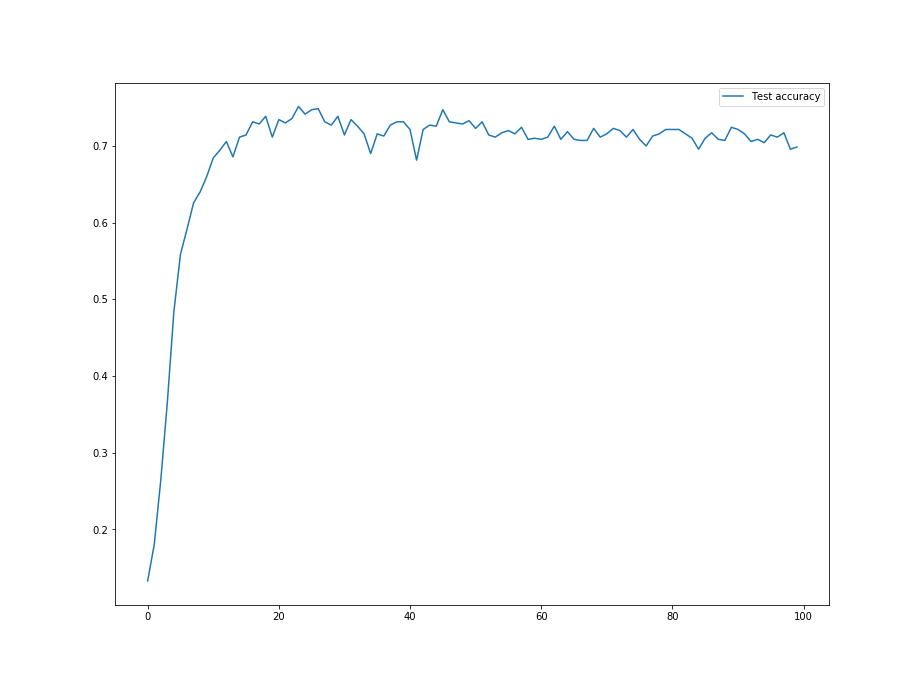
\includegraphics[width=1\linewidth]{assets/plots2/q3_2.png}
        \caption{Test accuracy against epochs for RNN}
        \label{fig:1a_cost}
    \end{subfigure}
    \caption{Plot of training cost and testing accuracy against epochs for Character RNN}
    \label{fig:1a}
\end{figure}


\subsection{Question 4}
\label{2q4}
\begin{quote}
Design a word RNN classifier that receives word ids and classify the input. The RNN is GRU layer and has a hidden-layer size of 20. Pass the inputs through an embedding layer of size 20 before feeding to the RNN. Plot the entropy on training data and the accuracy on testing data versus training epochs.
\end{quote}
\begin{figure}[H]
    \begin{subfigure}{0.5\textwidth}
        \centering
        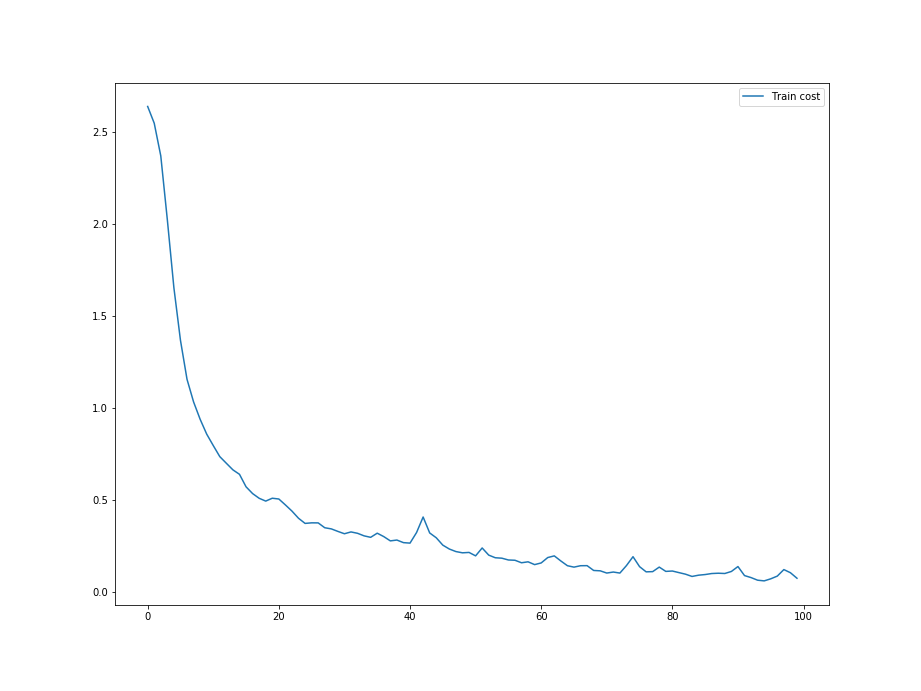
\includegraphics[width=1\linewidth]{assets/plots2/q3_1.png}
        \caption{Training cost against epochs for RNN}
    \end{subfigure}
    \begin{subfigure}{0.5\textwidth}
        \centering
        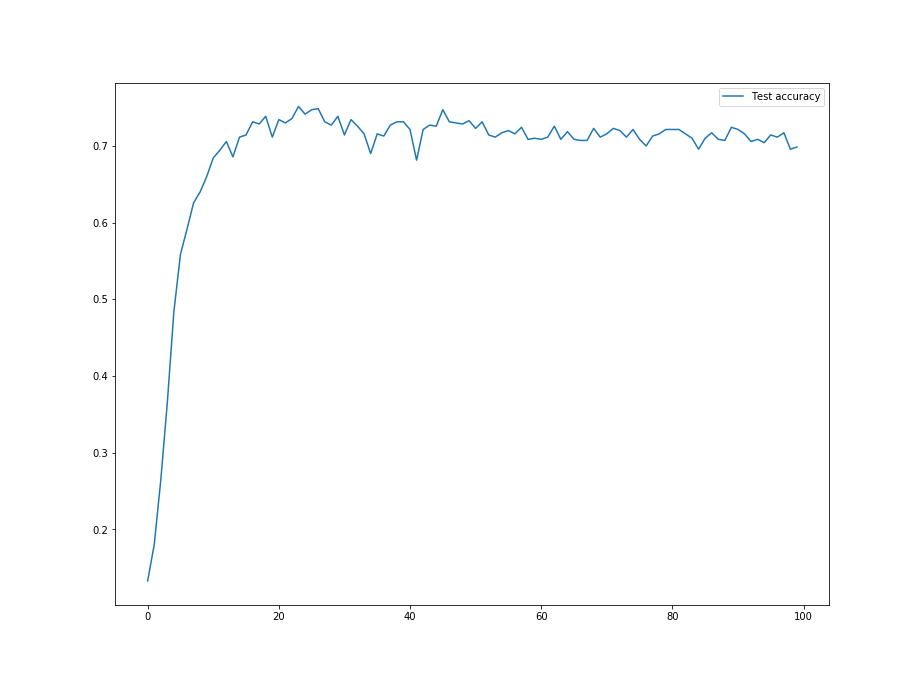
\includegraphics[width=1\linewidth]{assets/plots2/q3_2.png}
        \caption{Test accuracy against epochs for RNN}
    \end{subfigure}
    \caption{Plot of training cost and testing accuracy against epochs for Word RNN}
    \label{fig:2_4_1}
\end{figure}

\subsection{Question 5}
\begin{quote}
Compare the test accuracies and the running times of the networks implemented in parts (1) – (4). Experiment with adding dropout to the layers of networks in parts (1) – (4), and report the test accuracies. Compare and comment on the accuracies of the networks with/without
dropout.
\end{quote}

\begin{figure}[H]
    \begin{subfigure}{0.5\textwidth}
        \centering
        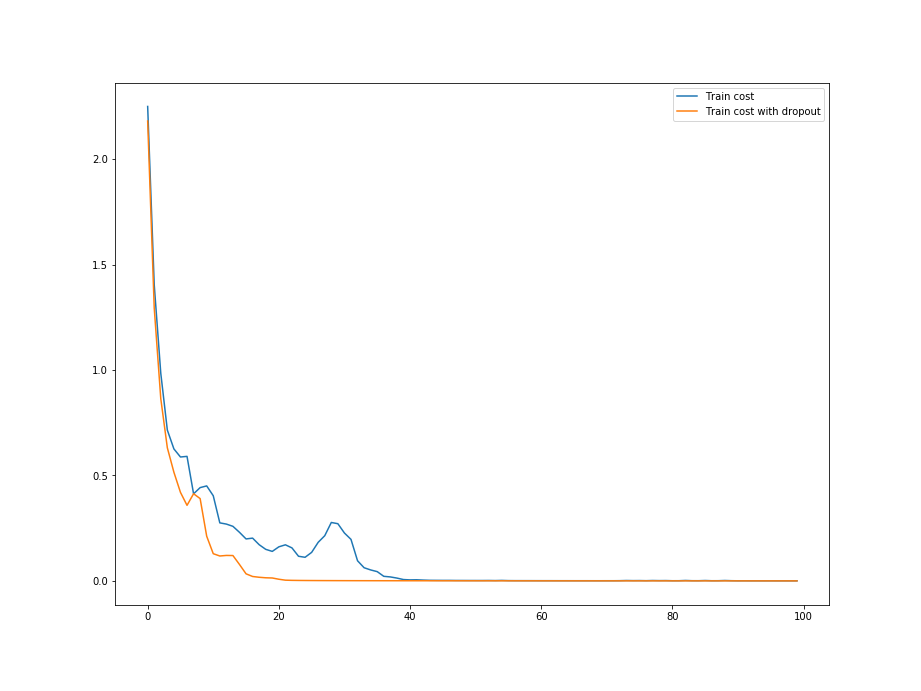
\includegraphics[width=1\linewidth]{assets/plots2/q1_3.png}
        \caption{Training cost against epochs for Character CNN}
    \end{subfigure}
    \begin{subfigure}{0.5\textwidth}
        \centering
        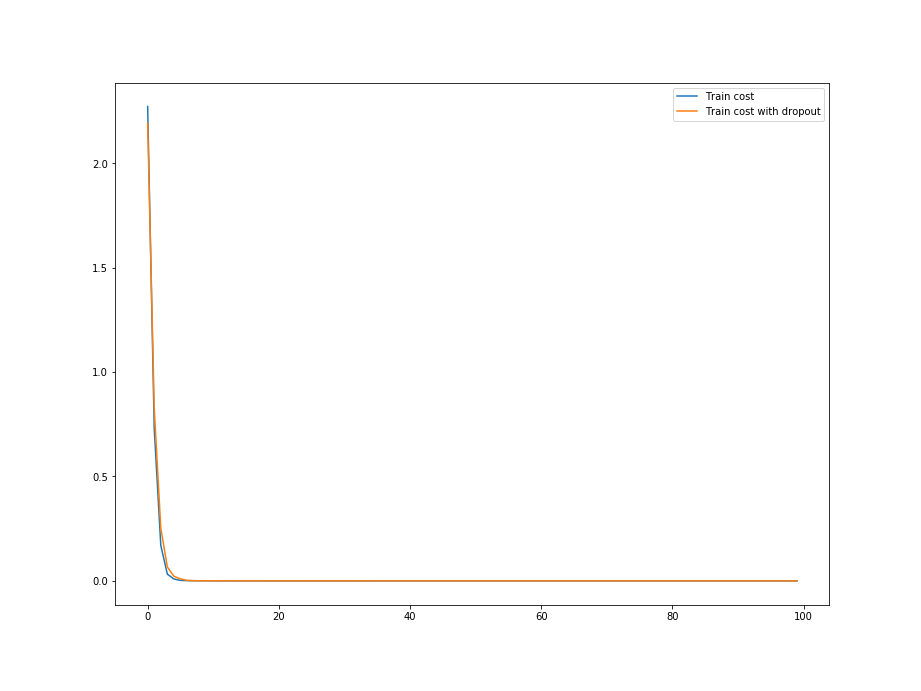
\includegraphics[width=1\linewidth]{assets/plots2/q2_3.png}
        \caption{Training cost against epochs for Word CNN}
    \end{subfigure}
    \begin{subfigure}{0.5\textwidth}
        \centering
        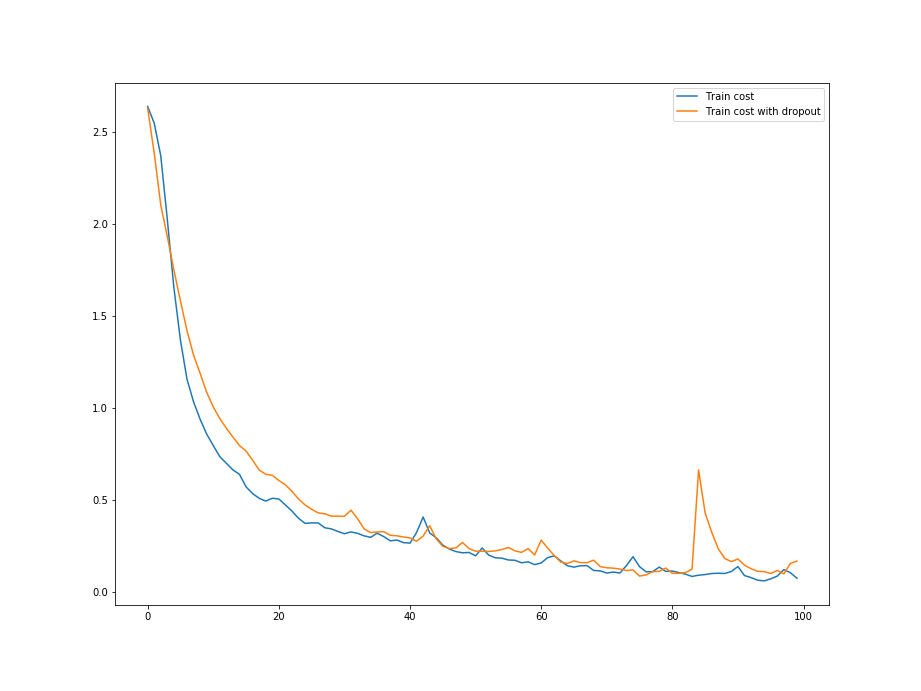
\includegraphics[width=1\linewidth]{assets/plots2/q3_3.png}
        \caption{Training cost against epochs for Character RNN}
    \end{subfigure}
    \begin{subfigure}{0.5\textwidth}
        \centering
        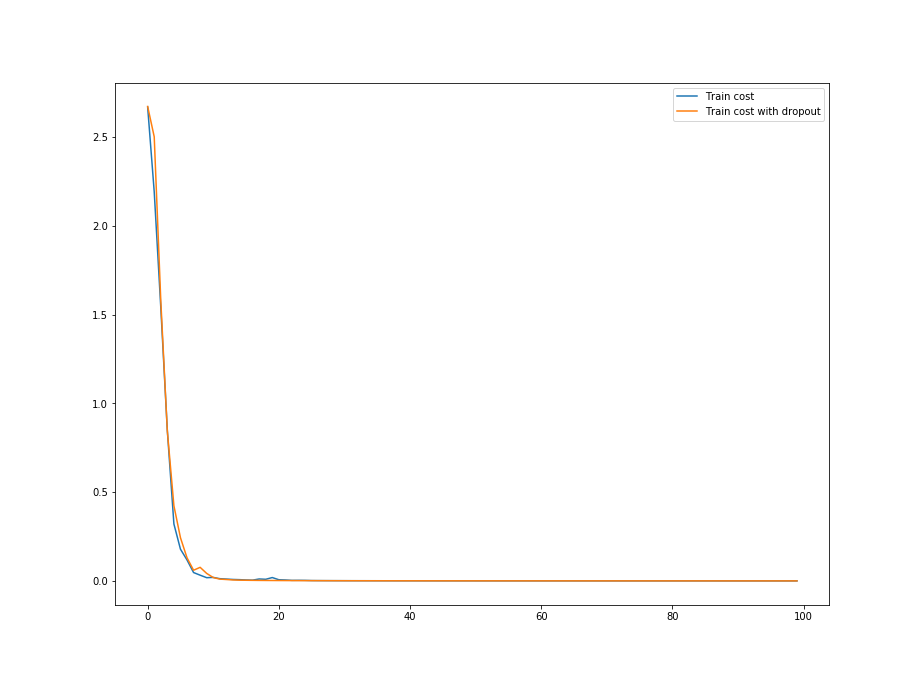
\includegraphics[width=1\linewidth]{assets/plots2/q4_3.png}
        \caption{Training cost against epochs for Word RNN}
    \end{subfigure}
    \caption{Dropout training cost comparisons for Charcter and Word classification for CNN and RNN}
    \label{fig:2_4_2}
\end{figure}

\begin{figure}[H]
    \begin{subfigure}{0.5\textwidth}
        \centering
        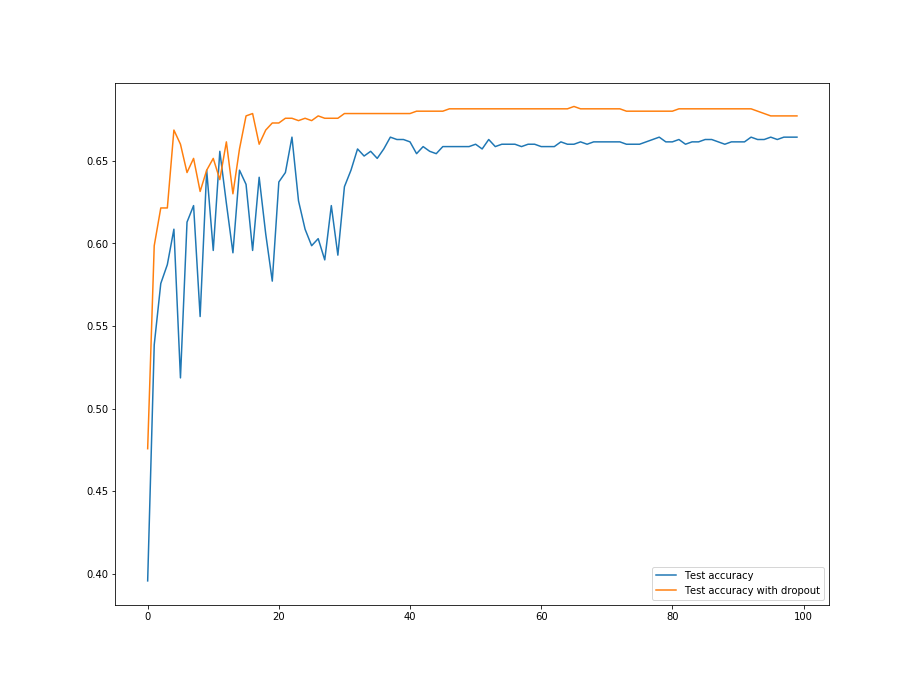
\includegraphics[width=1\linewidth]{assets/plots2/q1_4.png}
        \caption{Test accuracy against epochs for Character CNN}
    \end{subfigure}
    \begin{subfigure}{0.5\textwidth}
        \centering
        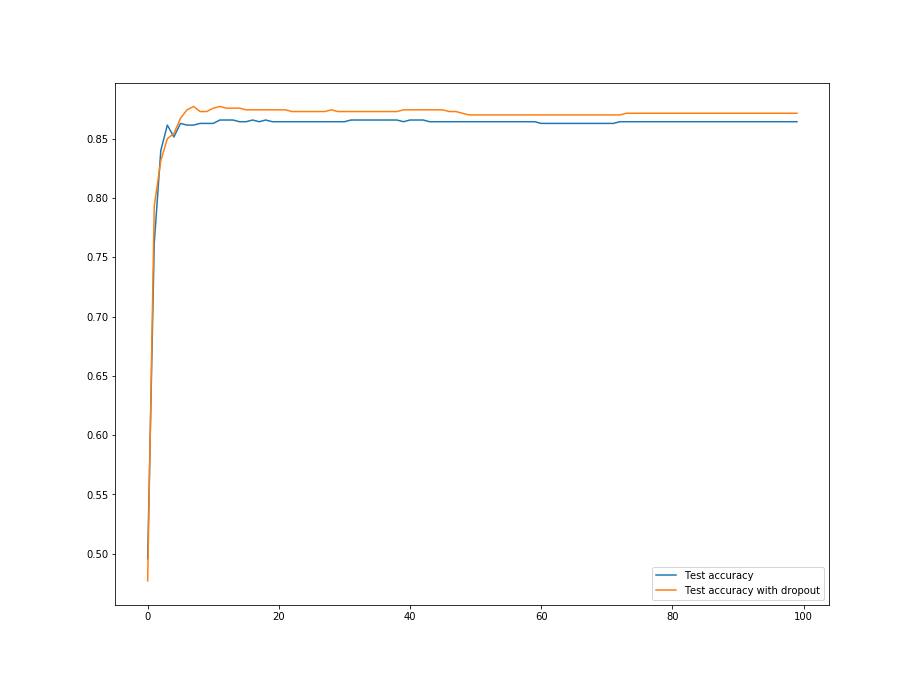
\includegraphics[width=1\linewidth]{assets/plots2/q2_4.png}
        \caption{Test accuracy against epochs for Word CNN}
    \end{subfigure}
    \begin{subfigure}{0.5\textwidth}
        \centering
        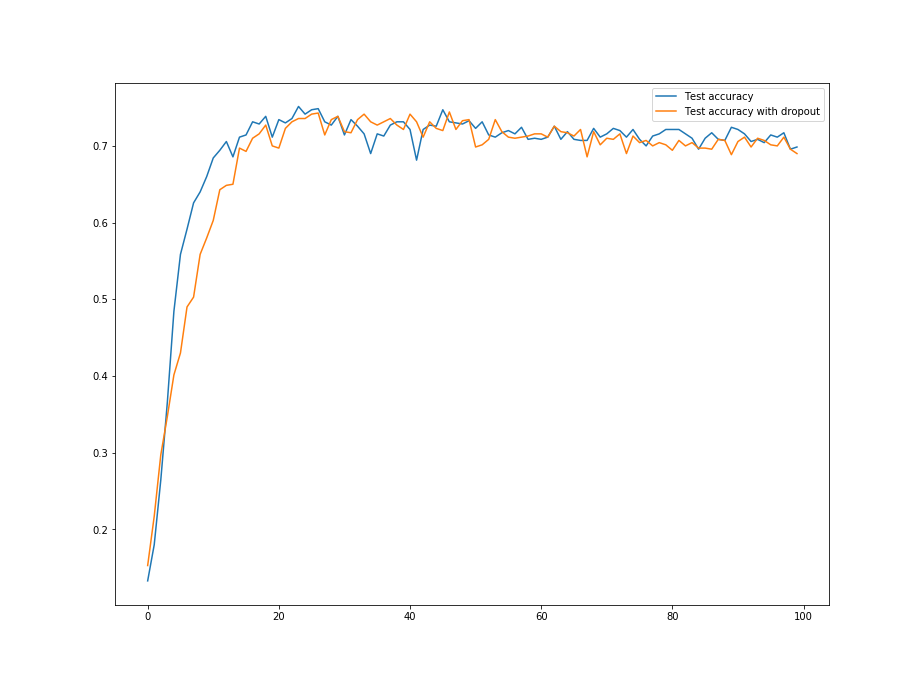
\includegraphics[width=1\linewidth]{assets/plots2/q3_4.png}
        \caption{Test accuracy against epochs for Character RNN}
    \end{subfigure}
    \begin{subfigure}{0.5\textwidth}
        \centering
        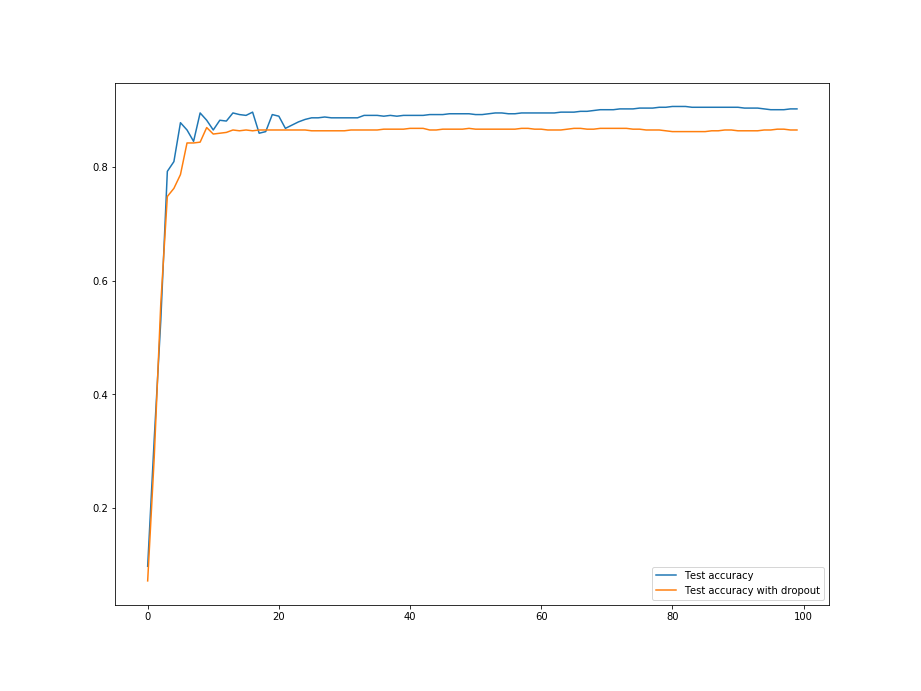
\includegraphics[width=1\linewidth]{assets/plots2/q4_4.png}
        \caption{Test accuracy against epochs for Word RNN}
    \end{subfigure}
    \caption{Dropout test accuracy comparisons for Charcter and Word classification for CNN and RNN}
    \label{fig:2_4_3}
\end{figure}

We initially experimented with a dropout rate of (0.1, 0.25, 0.25, 0.5), similar to the dropouts used in \cite{srivastava2014dropout} but achieved accuracy lesser with dropout. This is due to the fact that placing drop out at the start reduces the chances of epochs being activated, cutting down the number of test epochs. Placing drop out at the end, we are not able to identify and correct errors caused by the dropout that was implemented before, hence lowering accuracy.  So we removed the input and output dropouts, retaining only a dropout rate of (0.25, 0.25) for CNN layers, which allowed us to get better results. While applying dropout to CNN, it is also said that for CNN dropout "still helps because it provides noisy inputs for the higher fully connected layers which prevents them from overfitting. " in \cite{srivastava2014dropout}. This finding is consistent with our experiment in Figure \ref{fig:2_4_3}.

\begin{table}[H]
\centering
\begin{tabular}{|c|c|c|c|}
\hline
\rowcolor[HTML]{85A4FF} 
char CNN & word CNN & char RNN & word RNN \\ \hline
45.56 & 25.04 & 202.97 & 265.86 \\ \hline
\end{tabular}
\caption{ Network running times}
\label{tab:run_time}
\end{table}

The run times for the different networks can be found in Table \ref{tab:run_time}. It can be seen that for char classification, the CNN network is around 5 times faster than the RNN network, while for the word CNN network, it is more than 10x faster than the word RNN network. However, the accuracy of the word CNN network is about 10\% more than the accuracy of the word RNN network as well, while the accuracy of the char CNN network is similar to the accuracy of the char RNN network.

\subsection{Question 6}
\begin{quote}
For RNN networks implemented in (3) and (4), perform the following experiments with the aim of improving performances, compare the accuracies and report your findings:

a. Replace the GRU layer with (i) a vanilla RNN layer and (ii) a LSTM layer

b. Increase the number of RNN layers to 2 layers

c. Add gradient clipping to RNN training with clipping threshold = 2. 
\end{quote}

\begin{figure}[H]
    \begin{subfigure}{0.5\textwidth}
        \centering
        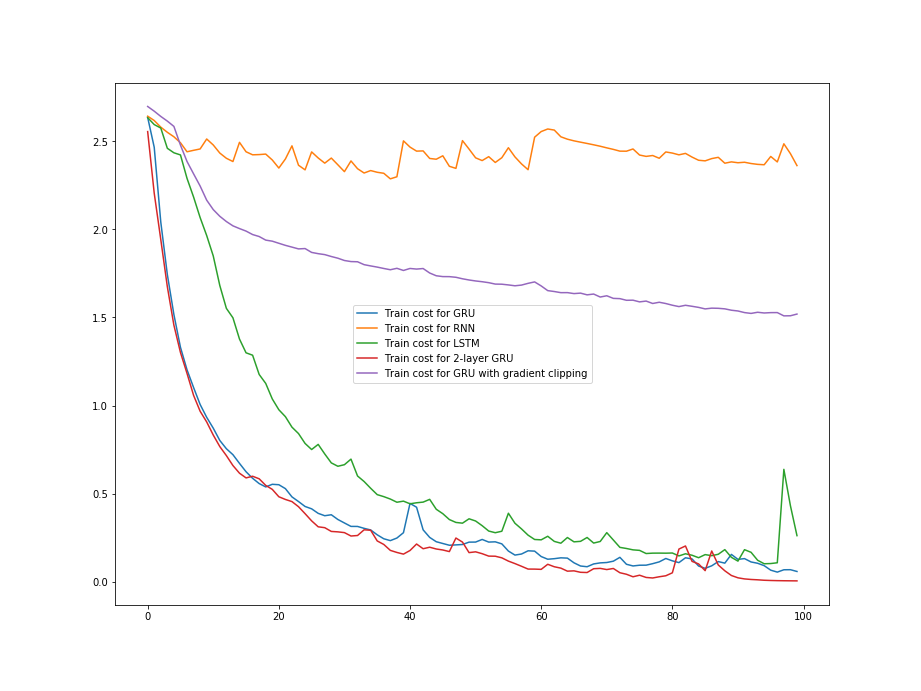
\includegraphics[width=1\linewidth]{assets/plots2/q6_1.png}
        \caption{Training cost for Character RNN}
    \end{subfigure}
    \begin{subfigure}{0.5\textwidth}
        \centering
        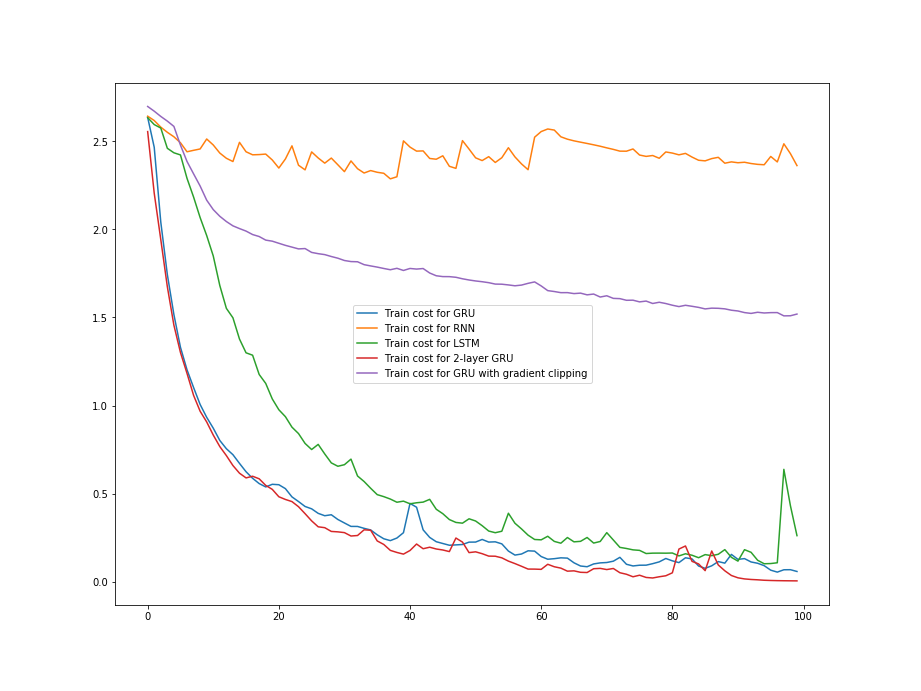
\includegraphics[width=1\linewidth]{assets/plots2/q6_3.png}
        \caption{Test accuracy cost for Character RNN}
    \end{subfigure}
    \begin{subfigure}{0.5\textwidth}
        \centering
        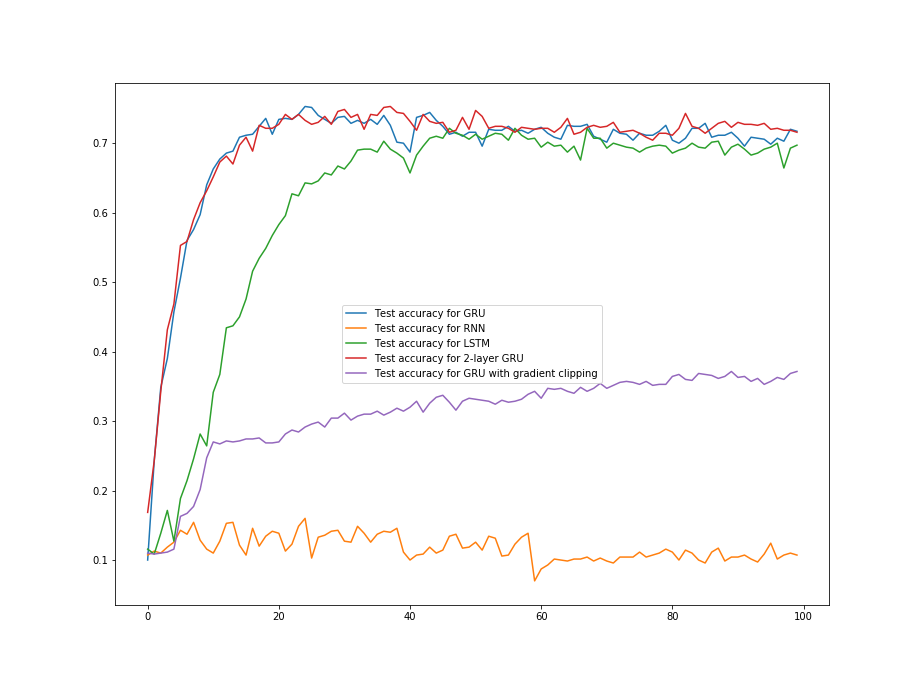
\includegraphics[width=1\linewidth]{assets/plots2/q6_2.png}
        \caption{Training cost for Word RNN}
    \end{subfigure}
    \begin{subfigure}{0.5\textwidth}
        \centering
        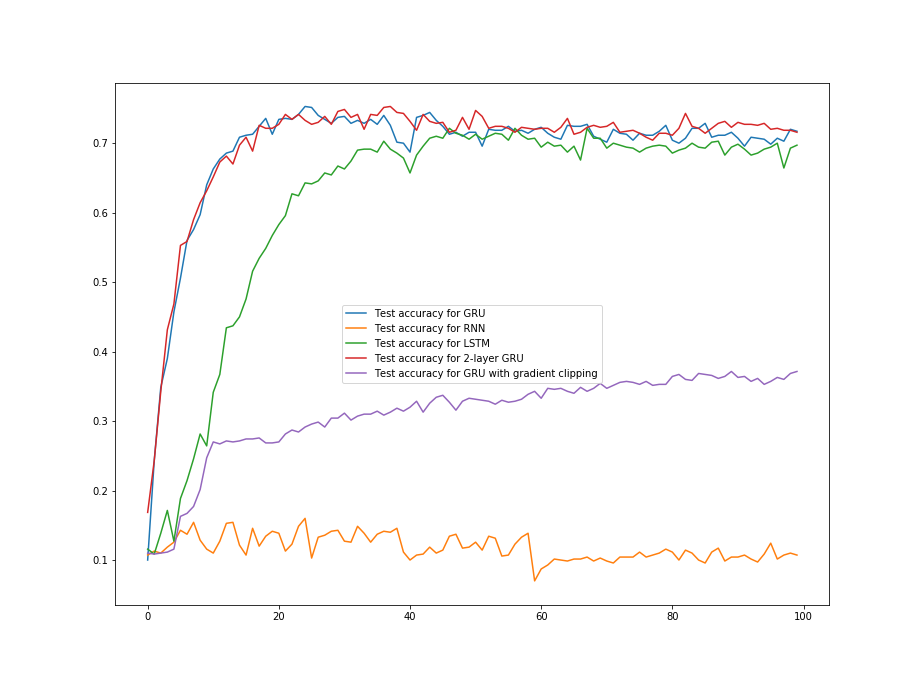
\includegraphics[width=1\linewidth]{assets/plots2/q6_4.png}
        \caption{Test accuracy cost for Word RNN}
    \end{subfigure}
    \caption{Plot of training cost and testing accuracy against epochs for different layer type, layers and gradient clipping}
    \label{fig:2_6}
\end{figure}

For this experiment, we are using the original GRU layer (blue in Figure \ref{fig:2_6}) as a benchmark/ control for result comparison.

\begin{enumerate}[label=(\alph*)]
    \item 
    \begin{enumerate}[label=(\roman*)]
        \item Having a vanilla RNN layer cause an extreme drop in accuracy and performance. This is because with each step, the content is overwritten. This makes it harder for the RNN to predict future outcomes based on past memory which will result in wrong predictions, thus having the worst performance.

        \item The LSTM layer has similar performance as the original GRU layer. This is due to the fact that having a LSTM layer allows the ability to retain or forget information, creating a control flow within the network. It allows for detection of an important input feature and carry it over long distances, thus it is capable of learning long-term dependencies. This reduces the chance of exploding gradient problems which is why it has similar performances as a GRU layer.
    \end{enumerate}
    
    \item Having the number of GRU layers increased to 2 resulted in better performance of the network as compared to using a single layer because having more layers allows for training of more complex arbitrary functions, thus doing a better job at predicting future outcomes resulting in better performance. This, as can be seen in Figure \ref{fig:2_6}, it had the best performance out of all the other setups.
    
    \item Gradient clipping forces the gradient values to specific maximum and minimum values if the gradient exceeds the given range. This method addresses the numerical stability of training deep neural network models and does not offer any general improvement in performance. The network converges slower but it can reach the accuracy of the other networks when given enough epoches. Since the gradient is limited within a range of 2.0, the results will also be limited thus it may not be as ideal as compared to the other networks, hence a drop in performance. However, on running a much higher number of epoches, the accuracy still increases to about the same accuracy as the other setups, which means that the introduction of gradient clipping actually greatly reduced the rate of convergence for our experiment.
\end{enumerate}

Therefore from the experiment, the vanilla RNN layer has the worst accuracy as compared to the others. Whereas, having 2 GRU layers resulted in the best performance

\section{Conclusion}
In conclusion, we have discussed two problems in this report and experienced the differences in utilizing different optimizers and techniques for a RNN in handling these 2 different problems.